%%%% ijcai19.tex

\typeout{IJCAI-19 Instructions for Authors}

% These are the instructions for authors for IJCAI-19.

\documentclass{article}
\pdfpagewidth=8.5in
\pdfpageheight=11in
% The file ijcai19.sty is NOT the same than previous years'
\usepackage{ijcai19}

% Use the postscript times font!
\usepackage{times}
\usepackage{soul}
\usepackage{url}
\usepackage[hidelinks]{hyperref}
\usepackage[utf8]{inputenc}
\usepackage[small]{caption}
\usepackage{graphicx}
\usepackage{amsmath}
\usepackage{booktabs}
\usepackage{algorithm}
\usepackage{algorithmic}
\urlstyle{same}

% the following package is optional:
%\usepackage{latexsym} 

% Following comment is from ijcai97-submit.tex:
% The preparation of these files was supported by Schlumberger Palo Alto
% Research, AT\&T Bell Laboratories, and Morgan Kaufmann Publishers.
% Shirley Jowell, of Morgan Kaufmann Publishers, and Peter F.
% Patel-Schneider, of AT\&T Bell Laboratories collaborated on their
% preparation.

% These instructions can be modified and used in other conferences as long
% as credit to the authors and supporting agencies is retained, this notice
% is not changed, and further modification or reuse is not restricted.
% Neither Shirley Jowell nor Peter F. Patel-Schneider can be listed as
% contacts for providing assistance without their prior permission.

% To use for other conferences, change references to files and the
% conference appropriate and use other authors, contacts, publishers, and
% organizations.
% Also change the deadline and address for returning papers and the length and
% page charge instructions.
% Put where the files are available in the appropriate places.

\title{Étiquetage de la race de chien depuis une image à l'aide d'un réseau de neurone convolutif}

% Single author syntax
\iffalse
\author{
    Sarit Kraus
    \affiliations
    Department of Computer Science, Bar-Ilan University, Israel \emails
    pcchair@ijcai19.org
}
\fi

% Multiple author syntax (remove the single-author syntax above and the \iffalse ... \fi here)
% Check the ijcai19-multiauthor.tex file for detailed instructions
\author{
Antoine Gaulin\and
Othman Mounir\and
Arthur Pulvéric\And
Anis Redjdal\\
\affiliations
Polytechnique Montréal\\
}

\begin{document}

\maketitle

\begin{abstract}
Décrire la thèse et le résultat en moins de 200 mots. Le document est de 6 pages maximum.
L'article a pour but de présenter un modèle de classification et d'étiquetage d'images
de chiens en fonction de leur race.
\end{abstract}

\section{Introduction}

\subsection{Motivations}

Les réseaux de neurones convolutifs permettent de faire de la classification d'image
de façon rapide et performante. Ainsi, avec des images de chiens, il est possible de
calculer la probabilité qu'un canidé présent dans une image appartienne à une race
plutôt qu’une autre. Pour aider la SPCA à se créer un inventaire en ligne de tous 
ses chiens, et encourager le commerce en ligne, nous voulons concevoir un réseau
de neurones qui permet de faire de la classification automatique à partir des images
de chien. De cette façon, les clients souhaitant faire l'acquisition d'une race
spécifique auront plus de facilité à la retrouver sur leur site internet.

Dans la pratique, un réseau de neurones convolutif classique présente des
difficultés pour la classification d’objets présentant de nombreuses caractéristiques
communes, ce qui est le cas pour les chiens de la base de données. La Fig. \ref{1}
illustre bien ce problème : les chiens présentés ont beaucoup de caractéristiques
communes, mais n’appartiennent pas à la même race. L’objectif ici est donc
d’implémenter un modèle capable d’obtenir des performances acceptables pour
la prédiction de races de chien.

\begin{figure}[htbp]
    \centering
    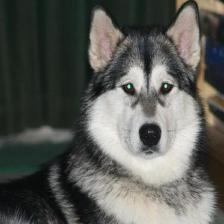
\includegraphics[width=2.8cm]{../dataset/test/n02110063-malamute/n02110063_11838.jpg}\hfill 
    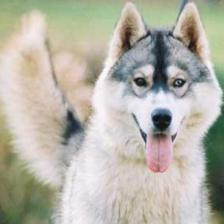
\includegraphics[width=2.8cm]{../dataset/test/n02109961-Eskimo_dog/n02109961_623.jpg}\hfill 
    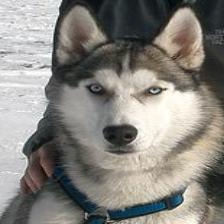
\includegraphics[width=2.8cm]{../dataset/test/n02110185-Siberian_husky/n02110185_7564.jpg} 
    \caption{De gauche à droite, un Malmute, un Eskimo et un Husky}
    \label{1} 
\end{figure} 

\subsection{Travaux antérieurs}
% Un petit résumé des travaux antérieurs qui existent dans la littérature.
L'article \textit{Using Convolutional Neural Networks to Classify Dog Breeds}
~\cite{fcdh_FinalReport} est un incontournable. Concrètement, les auteurs
proposent  deux architectures différentes capables de différencier les petites
variations entre les races. Le premier modèle est basé sur l'architecture de LeNet,
dont chaque couche de convolution est un filtre avec 2 paramètres : le nombre de
pixels qu’elles prennent en entrée et le nombre de canaux en sortie. Le deuxième
modèle reprend l'architecture de GoogLeNet, dont chaque couche de convolution
est une combinaison de filtres eux-mêmes composés de réseaux de neurones.

Un autre papier intéressant est \textit{Dog Breed Identification}. ~\cite{output} Il 
y est présenté un projet ayant pour but de prédire les races des chiens à partir
d’images. Ce projet utilise des techniques d’apprentissage automatique et de vision
par ordinateur. Un réseau de neurones convolutionnel permet dans un premier
temps d’identifier les points clés des visages des chiens. Ensuite, des descripteurs
SIFT (Scale-Invariant Feature Transform) et des histogrammes de couleur utilisent 
ces points clés pour extraire des features. Enfin, un classificateur de type machine 
à vecteur de support (SVM, Support-Vector Machine) prédit la race du chien avec
une précision de 52\%. Il est à noter que dans 90\% des cas, la race du chien à 
trouver est présente dans les 10 prédictions les plus probables (sur 133 races au
total dans la base de données). Ces performances sont supérieures à ce que
peuvent faire la plupart des humains.

Dans ce travail, nous faisons le choix d'utiliser un modèle proposé par le premier
article. En effet, la simplicité d’architecture et leurs bonnes performances sont
totalement adaptées aux contraintes que nous rencontrons. Nous allons ajouter un
algorithme qui applique une étiquette sur l'image.

\section{Approche théorétique}
% Un résumé de l'approche théorétique formant la base du sujet du projet.
Dans le contexte de la pandémie, nous devons limiter le projet à quelque chose de
simple, qui permet toutefois de comprendre le fonctionnement d'un CNN moderne en profondeur. Ainsi, nous allons nous limiter à une seule architecture.

Premièrement, nous avons évalué s'il était possible d'ajouter des étiquettes à une
image dans ses métadonnées à l'aide du langage Python. Nous avons trouvé la
librairie IPTCInfo qui permet de faire cette tâche aisément.

Ensuite, nous avons cherché un dataset pour entrainer notre modèle. Les images
retenues proviennent du \textit{Stanford Dogs Dataset}. 
~\cite{KhoslaYaoJayadevaprakashFeiFei_FGVC2011} Le fait que les clichés soient
présents dans des répertoires nommés par la race permet facilement de retrouver
l'étiquette pour faire l'entrainement supervisé. 

Avant de faire une architecture plus difficile, nous avons commencé par un réseau CNN de base.

\section{Discussion}

Discussion de nos expériences. Incluant des figures, des tableaux de nos résultats.

Le code source est disponible à cette adresse : \url{https://github.com/Anteige/INF8225}.

\subsection{Exemples de tableau}

\begin{table}[htbp]
\centering
\begin{tabular}{lrr}  
\toprule
Scenario  & $\delta$ (s) & Runtime (ms) \\
\midrule
Paris       & 0.1  & 13.65      \\
            & 0.2  & 0.01       \\
New York    & 0.1  & 92.50      \\
Singapore   & 0.1  & 33.33      \\
            & 0.2  & 23.01      \\
\bottomrule
\end{tabular}
\caption{Booktabs table}
\label{tab:booktabs}
\end{table}

\subsection{Exemple d'algorithme}

\begin{algorithm}[htbp]
\caption{Example algorithm}
\label{alg:algorithm}
\textbf{Input}: Your algorithm's input\\
\textbf{Parameter}: Optional list of parameters\\
\textbf{Output}: Your algorithm's output
\begin{algorithmic}[1] %[1] enables line numbers
\STATE Let $t=0$.
\WHILE{condition}
\STATE Do some action.
\IF {conditional}
\STATE Perform task A.
\ELSE
\STATE Perform task B.
\ENDIF
\ENDWHILE
\STATE \textbf{return} solution
\end{algorithmic}
\end{algorithm}

\subsection{Exemple de formule}

\begin{align}
    x =& \prod_{i=1}^n \sum_{j=1}^n j_i + \prod_{i=1}^n \sum_{j=1}^n i_j + \prod_{i=1}^n \sum_{j=1}^n j_i + \prod_{i=1}^n \sum_{j=1}^n i_j + \nonumber\\
    + & \prod_{i=1}^n \sum_{j=1}^n j_i
\end{align}

\section{Analyse}

Une analyze critique de l'approche que vous avez utilisée pour apprendre le sujet que vous avez sélectionné.


%% The file named.bst is a bibliography style file for BibTeX 0.99c
\bibliographystyle{named}
\bibliography{rapport}

\end{document}

